\chapter{Requirements Engineering for Embedded Systems}
\label{app:requirements}
\index{requirements engineering|(}

Requirements engineering is the foundation of successful system development. Before we can build, simulate, or verify a cyber-physical system, we must understand what it should do. This appendix covers the essential practices for collecting, analyzing, documenting, and managing requirements for embedded systems.

\section{Why Requirements Matter}

Studies consistently show that requirements errors are among the most costly defects in system development:

\begin{itemize}
    \item 50--60\% of all software defects can be traced to requirements problems
    \item Requirements errors discovered during testing cost 10--100 times more to fix than those found during requirements analysis
    \item Requirements errors discovered in deployed systems cost 100--1000 times more
\end{itemize}

For cyber-physical systems, the stakes are even higher. A missing or incorrect requirement can lead to:

\begin{itemize}
    \item Safety hazards (incorrect behavior under failure conditions)
    \item Certification failure (missing required functionality)
    \item Costly redesign (discovering timing constraints cannot be met)
    \item Field failures (environmental conditions not anticipated)
\end{itemize}

\begin{keyidea}
Verification can only prove that you built what you specified. It cannot prove that you specified the right thing. Requirements engineering is where you determine the ``right thing.''
\end{keyidea}

\subsection{Requirements in the Development Process}

Requirements serve as the contract between stakeholders and developers. They answer the fundamental question: \emph{What should this system do?} The development process then addresses \emph{how} to achieve those requirements through design, implementation, and verification.

\begin{center}
\begin{tikzpicture}[every node/.style={font=\small}]
    % Boxes
    \node[draw, rectangle, rounded corners, fill=blue!15, minimum width=2.5cm, minimum height=1cm, align=center] (stake) at (0, 0) {Stakeholder\\Needs};
    \node[draw, rectangle, rounded corners, fill=green!15, minimum width=2.5cm, minimum height=1cm, align=center] (req) at (4, 0) {Requirements};
    \node[draw, rectangle, rounded corners, fill=yellow!15, minimum width=2.5cm, minimum height=1cm, align=center] (design) at (8, 0) {Design \&\\Implementation};
    \node[draw, rectangle, rounded corners, fill=red!15, minimum width=2.5cm, minimum height=1cm, align=center] (verify) at (12, 0) {Verification};

    % Arrows
    \draw[-{Stealth}, thick] (stake) -- (req) node[midway, above] {\scriptsize elicit};
    \draw[-{Stealth}, thick] (req) -- (design) node[midway, above] {\scriptsize implement};
    \draw[-{Stealth}, thick] (design) -- (verify) node[midway, above] {\scriptsize verify};

    % Feedback
    \draw[-{Stealth}, dashed, gray] (verify.south) -- ++(0, -0.8) -| (req.south) node[midway, below] {\scriptsize validate};
\end{tikzpicture}
\end{center}

For CPS, requirements must capture aspects from multiple domains:
\begin{itemize}
    \item \textbf{Physical behavior}: How the system interacts with the physical world
    \item \textbf{Timing constraints}: When things must happen
    \item \textbf{Safety properties}: What must never happen
    \item \textbf{Resource limits}: Memory, power, weight, cost constraints
\end{itemize}

\section{Requirements Elicitation}
\index{requirements elicitation}

\emph{Elicitation} is the process of discovering and gathering requirements from stakeholders and other sources. It is often the most challenging phase because stakeholders may not know exactly what they need, may have conflicting needs, or may express needs in terms of solutions rather than problems.

\subsection{Stakeholder Identification}
\index{stakeholder}

The first step is identifying who has requirements. For a quadrotor system, stakeholders might include:

\begin{center}
\begin{tabular}{ll}
\toprule
\textbf{Stakeholder} & \textbf{Example Concerns} \\
\midrule
Pilot/Operator & Responsiveness, ease of control, flight time \\
Safety Officer & Failure modes, emergency procedures, containment \\
Maintenance Technician & Diagnostics, repairability, component access \\
Regulatory Authority & Airworthiness, operational limits, documentation \\
Manufacturer & Cost, manufacturability, warranty \\
General Public & Noise, privacy, safety from falling drones \\
\bottomrule
\end{tabular}
\end{center}

Each stakeholder brings different perspectives and constraints. Missing a stakeholder early often means discovering their requirements late, when changes are expensive.

\subsection{Elicitation Techniques}

Several techniques help extract requirements from stakeholders:

\paragraph{Interviews and Workshops}
Direct conversations with stakeholders are the most common technique. Structured interviews follow a prepared list of questions; unstructured interviews allow free-form discussion. Workshops bring multiple stakeholders together to discuss and negotiate requirements.

\paragraph{Observation and Domain Analysis}
Watching users operate similar systems reveals implicit requirements that users cannot articulate. Domain analysis studies the problem space---physics, regulations, existing solutions---to identify constraints.

\paragraph{Prototyping and Simulation}
Early prototypes help stakeholders understand possibilities and refine their needs. Simulation allows exploring ``what if'' scenarios before committing to requirements.

\paragraph{Scenario-Based Elicitation}
\index{use case}
Use cases describe how users interact with the system to achieve goals. Misuse cases describe how the system might be used incorrectly or maliciously, revealing safety and security requirements.

\begin{example}[Quadrotor Use Case]
\textbf{Use Case}: Automated Landing

\textbf{Primary Actor}: Pilot

\textbf{Preconditions}: Quadrotor is in flight, battery above 10\%

\textbf{Main Success Scenario}:
\begin{enumerate}
    \item Pilot initiates landing command
    \item System confirms safe landing zone below
    \item System descends at controlled rate
    \item System detects ground contact
    \item System disarms motors
\end{enumerate}

\textbf{Extensions}:
\begin{itemize}
    \item 2a. No safe landing zone: System alerts pilot, maintains hover
    \item 3a. Obstacle detected during descent: System pauses, alerts pilot
    \item 4a. Ground contact not detected within timeout: System performs emergency motor cutoff
\end{itemize}
\end{example}

\subsection{Common Elicitation Pitfalls}

Several traps await the unwary requirements engineer:

\paragraph{Solutions Disguised as Requirements}
Stakeholders often state solutions rather than needs: ``The system shall use a Kalman filter'' instead of ``The system shall estimate attitude with error less than 2 degrees.'' The solution may be appropriate, but the requirement should express the need, leaving solution choice to design.

\paragraph{Implicit Assumptions}
Stakeholders assume certain things are ``obvious'' and do not state them. The quadrotor ``obviously'' should not fly into walls, but unless this is stated as a requirement, it may not be tested.

\paragraph{Conflicting Requirements}
Different stakeholders want incompatible things. The pilot wants maximum agility; the safety officer wants conservative limits. These conflicts must be identified and resolved, not ignored.

\paragraph{Vague Requirements}
``The system shall be reliable'' or ``The system shall respond quickly'' are not requirements---they are wishes. Requirements must be specific enough to be testable.

\begin{warningbox}
If you cannot describe a test that would verify a requirement, the requirement is not well-defined. Every requirement should have a corresponding verification method.
\end{warningbox}

\section{Requirements Categories}

Requirements for embedded systems fall into several categories, each requiring different elicitation and verification approaches.

\subsection{Functional Requirements}
\index{functional requirements}

Functional requirements describe what the system must \emph{do}---its behavior and capabilities:

\begin{itemize}
    \item \textbf{Input-output relationships}: ``When the pilot commands roll right, the quadrotor shall bank right.''
    \item \textbf{Operating modes}: ``The system shall support manual, assisted, and autonomous flight modes.''
    \item \textbf{State transitions}: ``The system shall transition from Armed to Flying when takeoff command is received and motors reach minimum thrust.''
    \item \textbf{Data processing}: ``The system shall fuse IMU and barometer data to estimate altitude.''
\end{itemize}

\subsection{Non-Functional Requirements}
\index{non-functional requirements}

Non-functional requirements describe \emph{how well} the system must perform:

\paragraph{Performance Requirements}
Quantitative measures of system behavior:
\begin{itemize}
    \item ``Attitude controller shall achieve 90\% settling time within 200~ms.''
    \item ``Position tracking error shall not exceed 0.5~m in steady state.''
    \item ``System shall process sensor data within 500~$\mu$s of acquisition.''
\end{itemize}

\paragraph{Safety Requirements}
\index{safety requirements}
Constraints that prevent harm:
\begin{itemize}
    \item ``Attitude shall not exceed 45 degrees from vertical during normal flight.''
    \item ``System shall initiate controlled descent if battery falls below 15\%.''
    \item ``Motors shall not spin while system is in disarmed state.''
\end{itemize}

\paragraph{Reliability Requirements}
Availability and failure characteristics:
\begin{itemize}
    \item ``System shall achieve mean time between failures of at least 1000 flight hours.''
    \item ``System shall detect sensor failures within 100~ms.''
    \item ``System shall remain controllable after single motor failure.''
\end{itemize}

\paragraph{Resource Requirements}
Constraints on system resources:
\begin{itemize}
    \item ``Flight controller software shall use no more than 128~KB RAM.''
    \item ``System shall operate for at least 7 minutes on full battery.''
    \item ``Total system weight shall not exceed 35~g.''
\end{itemize}

\paragraph{Environmental Requirements}
Operating conditions:
\begin{itemize}
    \item ``System shall operate in ambient temperatures from 0 to 40$^\circ$C.''
    \item ``System shall withstand wind gusts up to 5~m/s.''
    \item ``System shall tolerate vibration levels specified in MIL-STD-810G.''
\end{itemize}

\subsection{Interface Requirements}

Interface requirements define how the system connects to its environment:

\paragraph{Hardware Interfaces}
\begin{itemize}
    \item ``IMU shall communicate via SPI at 10~MHz clock rate.''
    \item ``Motors shall accept PWM signals with 400~Hz update rate.''
    \item ``Radio receiver shall provide CPPM signal on designated pin.''
\end{itemize}

\paragraph{Software Interfaces}
\begin{itemize}
    \item ``Attitude controller shall accept setpoints as quaternions.''
    \item ``Logging module shall output data in MAVLink format.''
    \item ``Ground station shall communicate via CRTP protocol.''
\end{itemize}

\paragraph{User Interfaces}
\begin{itemize}
    \item ``LED shall indicate system state: solid = ready, blinking = low battery.''
    \item ``System shall emit audio warning when battery reaches 20\%.''
\end{itemize}

\subsection{Regulatory Requirements}

For certified systems, regulations impose additional requirements:

\paragraph{Standards Compliance}
\begin{itemize}
    \item ``Software shall be developed in compliance with DO-178C, Design Assurance Level C.''
    \item ``System shall meet electromagnetic compatibility requirements of EN 55032.''
\end{itemize}

\paragraph{Documentation Requirements}
\begin{itemize}
    \item ``All requirements shall be uniquely identified and traceable to tests.''
    \item ``Design decisions shall be documented with rationale.''
\end{itemize}

\paragraph{Derived Requirements}
When a design decision creates new requirements, these are \emph{derived requirements}. For example, if the design uses a particular sensor with specific calibration needs, this creates derived requirements for calibration procedures. Derived requirements must be traced to their source and verified like original requirements.

\section{Requirements Analysis}

Once requirements are gathered, they must be analyzed for quality before being used as the basis for design.

\subsection{Completeness Analysis}

A requirements set is complete if it covers all necessary aspects of the system. Techniques for checking completeness include:

\paragraph{Checklists}
Standard lists of requirement categories ensure nothing is forgotten. For embedded systems, check for:
\begin{itemize}
    \item All operating modes defined
    \item All state transitions specified
    \item Startup and shutdown behavior
    \item Error handling and recovery
    \item Boundary conditions and edge cases
\end{itemize}

\paragraph{Traceability to Sources}
\index{traceability!requirements}
Every stakeholder need should trace to at least one requirement. If a need has no corresponding requirement, something is missing.

\paragraph{Coverage of Hazards}
Every identified hazard should trace to safety requirements that mitigate it.

\subsection{Consistency Analysis}

Requirements are consistent if they do not contradict each other. Inconsistencies arise from:

\begin{itemize}
    \item \textbf{Direct contradiction}: ``System shall respond within 10~ms'' vs. ``System shall complete all checks before responding'' (if checks take 20~ms)
    \item \textbf{Resource conflicts}: Requirements that together exceed available resources
    \item \textbf{Timing conflicts}: Requirements with incompatible timing constraints
\end{itemize}

Detecting inconsistencies early prevents discovering them during integration when fixes are expensive.

\subsection{Feasibility Analysis}

Some requirements may be technically impossible or prohibitively expensive. Feasibility analysis identifies these early:

\paragraph{Technical Feasibility}
Can the requirement be achieved with available technology? For example, requiring 0.01 degree attitude accuracy may exceed what affordable sensors can achieve.

\paragraph{Resource Feasibility}
Do the requirements fit within resource budgets? Add up all timing requirements to check if the processor can execute everything. Add up all memory requirements to check if they fit in available RAM.

\paragraph{Schedule and Cost Feasibility}
Can the requirements be met within project constraints? Some requirements may be deferrable to later versions.

\subsection{Safety Analysis Connection}

Safety analysis techniques identify hazards and trace them to safety requirements:

\paragraph{FMEA (Failure Mode and Effects Analysis)}
\index{FMEA (Failure Mode and Effects Analysis)}
For each component, identify how it can fail and what effects each failure has. Each significant effect generates a safety requirement to detect, mitigate, or prevent the failure.

\begin{example}[FMEA to Requirement]
\textbf{Component}: Motor 1

\textbf{Failure Mode}: Motor stops spinning

\textbf{Effect}: Loss of thrust, uncontrolled descent

\textbf{Severity}: Critical

\textbf{Derived Safety Requirement}: SR-101: System shall detect motor failure within 50~ms and initiate controlled descent using remaining motors.
\end{example}

\paragraph{FTA (Fault Tree Analysis)}
\index{FTA (Fault Tree Analysis)}
Start from an undesired event (the ``top event'') and work backward to identify combinations of failures that could cause it. Each path through the tree suggests requirements to break the causal chain.

\begin{center}
\begin{tikzpicture}[
    every node/.style={font=\small},
    event/.style={draw, rectangle, minimum width=2cm, minimum height=0.8cm, align=center},
    gate/.style={draw, trapezium, trapezium left angle=70, trapezium right angle=110, minimum width=1cm}
]
    % Top event
    \node[event, fill=red!20] (top) at (0, 0) {Uncontrolled\\Descent};

    % OR gate
    \node[gate] (or1) at (0, -1.5) {OR};

    % Second level
    \node[event] (e1) at (-3, -3) {Total Power\\Loss};
    \node[event] (e2) at (0, -3) {Control\\Failure};
    \node[event] (e3) at (3, -3) {Structural\\Failure};

    % Connections
    \draw (top) -- (or1);
    \draw (or1.south) -- ++(-3, -0.5) -- (e1);
    \draw (or1.south) -- (e2);
    \draw (or1.south) -- ++(3, -0.5) -- (e3);

    % Derived requirements
    \node[right of=e1, xshift=0.5cm, font=\scriptsize\itshape, align=left] {$\rightarrow$ Battery\\monitoring};
    \node[right of=e2, xshift=0.5cm, font=\scriptsize\itshape, align=left] {$\rightarrow$ Redundant\\sensors};
\end{tikzpicture}
\end{center}

\section{Requirements Documentation}

Well-documented requirements are unambiguous, testable, and traceable.

\subsection{Anatomy of a Good Requirement}

Each requirement should be:

\paragraph{Unambiguous}
Only one interpretation is possible. Avoid words like ``appropriate,'' ``sufficient,'' ``fast,'' or ``user-friendly'' without quantification.

\paragraph{Testable}
A clear test can determine whether the requirement is satisfied. ``Attitude error shall be less than 5 degrees'' is testable; ``Attitude control shall be accurate'' is not.

\paragraph{Atomic}
Each requirement expresses one capability. ``System shall track position and log data'' should be two requirements.

\paragraph{Feasible}
The requirement can be implemented with available resources and technology.

\paragraph{Traceable}
The requirement has a unique identifier and links to its source and verification.

\subsection{Requirement Language}

Standards like IEEE~830 recommend specific language patterns:

\begin{itemize}
    \item \textbf{``Shall''} indicates a mandatory requirement: ``The system \emph{shall} maintain attitude within 30 degrees.''
    \item \textbf{``Should''} indicates a goal that is desirable but not mandatory: ``The system \emph{should} achieve settling time under 100~ms.''
    \item \textbf{``May''} indicates an optional feature: ``The system \emph{may} support multiple radio protocols.''
\end{itemize}

\begin{notebox}
Consistent use of ``shall,'' ``should,'' and ``may'' makes requirements easier to prioritize and verify. Mixing these arbitrarily causes confusion about what is actually required.
\end{notebox}

\subsection{Documentation Structure}

Requirements should be organized hierarchically:

\begin{center}
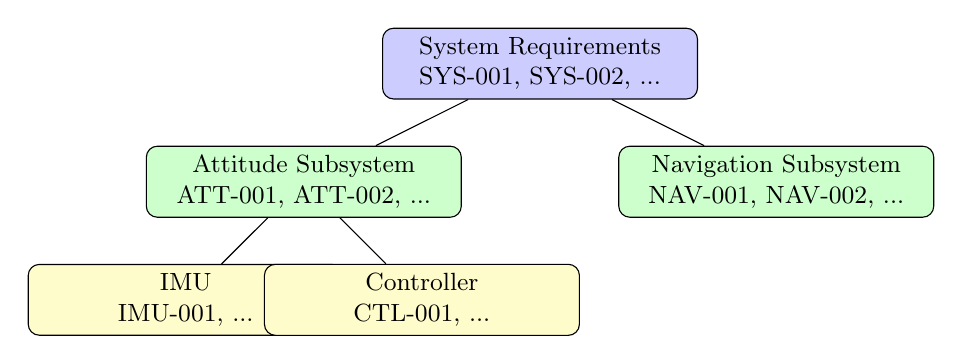
\begin{tikzpicture}[
    every node/.style={font=\small},
    level/.style={draw, rectangle, rounded corners, minimum width=4cm, minimum height=0.8cm, align=center}
]
    \node[level, fill=blue!20] (sys) at (0, 0) {System Requirements\\SYS-001, SYS-002, ...};
    \node[level, fill=green!20] (sub1) at (-3, -1.5) {Attitude Subsystem\\ATT-001, ATT-002, ...};
    \node[level, fill=green!20] (sub2) at (3, -1.5) {Navigation Subsystem\\NAV-001, NAV-002, ...};
    \node[level, fill=yellow!20] (comp1) at (-4.5, -3) {IMU\\IMU-001, ...};
    \node[level, fill=yellow!20] (comp2) at (-1.5, -3) {Controller\\CTL-001, ...};

    \draw (sys) -- (sub1);
    \draw (sys) -- (sub2);
    \draw (sub1) -- (comp1);
    \draw (sub1) -- (comp2);
\end{tikzpicture}
\end{center}

Each requirement should include:

\begin{itemize}
    \item \textbf{Identifier}: Unique ID (e.g., ATT-017)
    \item \textbf{Title}: Brief descriptive name
    \item \textbf{Description}: Full requirement statement using ``shall''
    \item \textbf{Rationale}: Why this requirement exists
    \item \textbf{Source}: Stakeholder need or parent requirement
    \item \textbf{Priority}: Must-have, should-have, nice-to-have
    \item \textbf{Verification method}: Test, analysis, inspection, or demonstration
\end{itemize}

\subsection{From Natural Language to Formal Specification}

Natural language requirements are readable but ambiguous. Formal specifications (like STL, covered in Module~4) are precise but harder to read. The bridge between them is crucial:

\begin{example}[Natural to Formal]
\textbf{Natural Language}: ``The attitude shall remain within safe limits during flight.''

\textbf{Refined Natural Language}: ``During flight, roll and pitch angles shall not exceed 30 degrees, and yaw rate shall not exceed 200 degrees per second.''

\textbf{Formal (STL)}: $\Box_{[0,T]}(|\phi| < 30° \land |\theta| < 30° \land |\dot{\psi}| < 200°/\text{s})$

where $\Box_{[0,T]}$ means ``always during interval $[0,T]$.''
\end{example}

Not all requirements need formal specification. Formalize requirements that:
\begin{itemize}
    \item Are safety-critical
    \item Will be checked by automated tools
    \item Have been ambiguous in the past
    \item Are complex enough that natural language is inadequate
\end{itemize}

\section{Requirements Traceability}

Traceability is the ability to follow requirements through the development process---from source through design, implementation, and testing.

\subsection{Why Traceability Matters}

Traceability serves multiple purposes:

\paragraph{Impact Analysis}
When a requirement changes, traceability shows which design elements, code, and tests are affected.

\paragraph{Completeness Verification}
Every requirement should trace to at least one test. If a requirement has no test, it may not be verified.

\paragraph{Certification Evidence}
Safety standards (DO-178C, ISO~26262) require traceability as evidence of development rigor.

\paragraph{Debugging}
When a test fails, traceability shows which requirement is violated, which helps identify the root cause.

\subsection{Traceability Matrix}

A traceability matrix shows relationships between requirements and other artifacts:

\begin{center}
\begin{tabular}{llll}
\toprule
\textbf{Req ID} & \textbf{Design Element} & \textbf{Code Module} & \textbf{Test Case} \\
\midrule
ATT-001 & Attitude Controller & attitude\_ctrl.c & TC-ATT-001 \\
ATT-002 & Rate Limiter & rate\_limit.c & TC-ATT-002 \\
ATT-003 & Motor Mixer & motor\_mix.c & TC-ATT-003a, TC-ATT-003b \\
NAV-001 & Position Estimator & pos\_est.c & TC-NAV-001 \\
\bottomrule
\end{tabular}
\end{center}

\begin{center}
\begin{tikzpicture}[every node/.style={font=\small}]
    % Requirements
    \node[draw, rectangle, fill=blue!20, minimum width=1.5cm] (r1) at (0, 2) {ATT-001};
    \node[draw, rectangle, fill=blue!20, minimum width=1.5cm] (r2) at (0, 1) {ATT-002};
    \node[draw, rectangle, fill=blue!20, minimum width=1.5cm] (r3) at (0, 0) {ATT-003};

    % Design
    \node[draw, rectangle, fill=green!20, minimum width=1.8cm] (d1) at (3.5, 1.5) {Controller};
    \node[draw, rectangle, fill=green!20, minimum width=1.8cm] (d2) at (3.5, 0) {Mixer};

    % Code
    \node[draw, rectangle, fill=yellow!20, minimum width=2cm] (c1) at (7, 1.5) {attitude\_ctrl.c};
    \node[draw, rectangle, fill=yellow!20, minimum width=2cm] (c2) at (7, 0) {motor\_mix.c};

    % Tests
    \node[draw, rectangle, fill=red!20, minimum width=1.5cm] (t1) at (10.5, 2) {TC-001};
    \node[draw, rectangle, fill=red!20, minimum width=1.5cm] (t2) at (10.5, 1) {TC-002};
    \node[draw, rectangle, fill=red!20, minimum width=1.5cm] (t3) at (10.5, 0) {TC-003};

    % Traces
    \draw[-{Stealth}] (r1) -- (d1);
    \draw[-{Stealth}] (r2) -- (d1);
    \draw[-{Stealth}] (r3) -- (d2);
    \draw[-{Stealth}] (d1) -- (c1);
    \draw[-{Stealth}] (d2) -- (c2);
    \draw[-{Stealth}] (c1) -- (t1);
    \draw[-{Stealth}] (c1) -- (t2);
    \draw[-{Stealth}] (c2) -- (t3);

    % Labels
    \node[above] at (0, 2.5) {\textbf{Requirements}};
    \node[above] at (3.5, 2.5) {\textbf{Design}};
    \node[above] at (7, 2.5) {\textbf{Code}};
    \node[above] at (10.5, 2.5) {\textbf{Tests}};
\end{tikzpicture}
\end{center}

\subsection{Tools for Requirements Management}

Industrial projects use specialized tools for requirements management:

\begin{itemize}
    \item \textbf{IBM DOORS}: Industry standard for large aerospace and automotive projects
    \item \textbf{Polarion}: Web-based ALM tool with requirements management
    \item \textbf{Jama Connect}: Requirements management with strong traceability
    \item \textbf{Simulink Requirements Toolbox}: Integrates requirements with Simulink models
\end{itemize}

For smaller projects, spreadsheets or issue trackers can provide basic traceability, though they lack the rigor of dedicated tools.

\section{Requirements Management}

Requirements are not static---they evolve throughout the project. Managing this evolution is critical.

\subsection{Change Management}

A change control process ensures that changes are deliberate and their impacts understood:

\begin{enumerate}
    \item \textbf{Request}: Stakeholder or engineer proposes a change
    \item \textbf{Impact analysis}: Identify affected design, code, and tests
    \item \textbf{Review}: Change control board evaluates cost/benefit
    \item \textbf{Approval/Rejection}: Decision recorded with rationale
    \item \textbf{Implementation}: If approved, update all affected artifacts
    \item \textbf{Verification}: Confirm change implemented correctly
\end{enumerate}

\begin{notebox}
``Just a small change'' is dangerous thinking. Even small requirement changes can have large impacts on safety-critical systems. Always trace the impact before approving.
\end{notebox}

\subsection{Versioning and Baselines}

Requirements should be version-controlled like code. Key concepts:

\paragraph{Baseline}
A frozen set of requirements at a specific point in time. Development phases often start with a baselined set of requirements.

\paragraph{Version History}
Each requirement should track its revision history, showing what changed and why.

\paragraph{Configuration Management}
Requirements, design, code, and tests should be managed together so their versions correspond.

\subsection{Requirements Reviews}

Formal reviews catch defects before they propagate:

\paragraph{Inspection}
Structured review where reviewers independently examine requirements, then meet to discuss findings. Studies show inspections find 60--90\% of defects.

\paragraph{Review Criteria}
Check that each requirement is:
\begin{itemize}
    \item Correct (accurately represents the need)
    \item Complete (no missing information)
    \item Unambiguous (only one interpretation)
    \item Consistent (no contradictions)
    \item Testable (verification method exists)
    \item Traceable (source identified)
\end{itemize}

\paragraph{Sign-off}
Stakeholders formally approve requirements before design proceeds. This creates accountability and a clear baseline.

\section{CPS-Specific Requirements Challenges}

Cyber-physical systems present unique requirements challenges that go beyond traditional software.

\subsection{Timing Requirements}

CPS must meet timing constraints, which must be captured as requirements:

\begin{itemize}
    \item \textbf{Period}: ``Attitude control shall execute every 2~ms $\pm$ 50~$\mu$s.''
    \item \textbf{Deadline}: ``Sensor processing shall complete within 500~$\mu$s of data arrival.''
    \item \textbf{Jitter}: ``Control loop period variation shall not exceed 100~$\mu$s.''
    \item \textbf{Latency}: ``End-to-end delay from sensor to actuator shall not exceed 3~ms.''
\end{itemize}

These requirements must be verifiable---typically through measurement on the actual hardware.

\subsection{Requirements Under Uncertainty}

CPS operate in uncertain environments. Requirements must account for this:

\paragraph{Robustness Requirements}
Specify performance bounds under disturbances:
\begin{itemize}
    \item ``System shall maintain position within 1~m despite wind gusts up to 5~m/s.''
    \item ``Attitude estimation error shall not exceed 5 degrees despite gyro bias of up to 1~deg/s.''
\end{itemize}

\paragraph{Probabilistic Requirements}
Some properties can only be guaranteed with probability:
\begin{itemize}
    \item ``Probability of successful landing shall exceed 99.9\%.''
    \item ``False alarm rate for obstacle detection shall not exceed 1 per hour.''
\end{itemize}

Verifying probabilistic requirements requires statistical testing.

\subsection{Requirements for Learning-Enabled Components}

As machine learning becomes common in CPS, new challenges arise:

\paragraph{Specification Challenges}
How do you specify what a neural network should do? Traditional input-output requirements may be insufficient for complex perception tasks.

\paragraph{Current Approaches}
\begin{itemize}
    \item \textbf{Operational Design Domain (ODD)}: Specify the conditions under which the system should operate correctly
    \item \textbf{Performance envelopes}: Specify bounds on error rates, response times, etc.
    \item \textbf{Safety monitors}: Specify runtime checks that can detect when the ML component is outside its competence
\end{itemize}

This is an active area of research with no complete solutions yet.

\section{Worked Example: Crazyflie Attitude Control Requirements}

This section demonstrates requirements engineering for the Crazyflie's attitude control subsystem.

\subsection{Stakeholders}

\begin{itemize}
    \item \textbf{Pilot}: Wants responsive, predictable control
    \item \textbf{Course instructor}: Wants safe operation in classroom environment
    \item \textbf{Developer}: Wants clear, testable specifications
\end{itemize}

\subsection{High-Level Requirements}

\begin{center}
\begin{tabular}{p{1.5cm}p{10cm}}
\toprule
\textbf{ID} & \textbf{Requirement} \\
\midrule
SYS-001 & The system shall provide attitude stabilization during flight. \\
SYS-002 & The system shall respond to pilot attitude commands within 200~ms. \\
SYS-003 & The system shall prevent attitudes that could cause loss of control. \\
\bottomrule
\end{tabular}
\end{center}

\subsection{Derived Requirements}

From SYS-001:
\begin{center}
\begin{tabular}{p{1.5cm}p{10cm}}
\toprule
\textbf{ID} & \textbf{Requirement} \\
\midrule
ATT-001 & The attitude controller shall execute at 500~Hz $\pm$ 1\%. \\
ATT-002 & Attitude estimation error shall not exceed 3 degrees RMS. \\
ATT-003 & IMU data shall be acquired within 100~$\mu$s of control loop start. \\
\bottomrule
\end{tabular}
\end{center}

From SYS-003:
\begin{center}
\begin{tabular}{p{1.5cm}p{10cm}}
\toprule
\textbf{ID} & \textbf{Requirement} \\
\midrule
SAF-001 & Roll and pitch angles shall not exceed 45 degrees during normal flight. \\
SAF-002 & Angular rates shall not exceed 300~deg/s on any axis. \\
SAF-003 & If attitude exceeds 60 degrees, system shall initiate emergency stop. \\
\bottomrule
\end{tabular}
\end{center}

\subsection{Formal Specifications}

Key requirements formalized in STL:

\textbf{SAF-001} (Attitude bounds):
$$\Box_{[0,T]}(|\phi| < 45° \land |\theta| < 45°)$$

\textbf{SYS-002} (Response time):
$$\Box_{[0,T]}\left(\text{cmd\_change} \Rightarrow \Diamond_{[0, 200\text{ms}]}(|\phi - \phi_{\text{cmd}}| < 5°)\right)$$

\subsection{Traceability}

\begin{center}
\begin{tabular}{llll}
\toprule
\textbf{Req} & \textbf{Source} & \textbf{Code} & \textbf{Test} \\
\midrule
ATT-001 & SYS-001 & stabilizer.c:42 & TC-ATT-001 \\
ATT-002 & SYS-001 & estimator.c:156 & TC-ATT-002 \\
SAF-001 & SYS-003 & stabilizer.c:89 & TC-SAF-001 \\
SAF-002 & SYS-003 & rate\_ctrl.c:34 & TC-SAF-002 \\
\bottomrule
\end{tabular}
\end{center}

\section{Summary}

Requirements engineering is the foundation of successful CPS development:

\begin{itemize}
    \item \textbf{Elicitation} discovers stakeholder needs through interviews, observation, prototyping, and scenario analysis
    \item \textbf{Categories} include functional, performance, safety, reliability, resource, environmental, interface, and regulatory requirements
    \item \textbf{Analysis} checks completeness, consistency, and feasibility before design begins
    \item \textbf{Documentation} makes requirements unambiguous, testable, and traceable
    \item \textbf{Traceability} connects requirements to design, code, and tests throughout development
    \item \textbf{Management} handles the inevitable changes with controlled processes
    \item \textbf{CPS challenges} include timing constraints, uncertainty, and learning-enabled components
\end{itemize}

\begin{keyidea}
Good requirements do not guarantee a good system, but bad requirements guarantee problems. Invest time in getting requirements right---it pays off throughout development.
\end{keyidea}

Requirements engineering connects directly to the verification techniques in Module~4: the formal specifications developed here become the properties checked by STL-based testing, and the traceability developed here demonstrates test coverage for certification.
\index{requirements engineering|)}
